Model-view-viewmodel (MVVM) is a software that helps to 
cleanly separate business and presentation logic of an
application from the its user interface (UI), \hl{making it
easier to test, maintain and evolve}. It can also \hl{code re-use}
opportunities and allows developers and UI designers to more 
\hl{easily collaborate} when developing their respective parts 
in the app. This is a famous pattern and used in \hl{Xamarim} and 
it is similar to the \textbf{MVP} (Model View Presenter) pattern, however
the drawbacks of the MVP has been solved.

\subsection{The MVVP Pattern}
The pattern is divided in three parts: the model, the view and the 
view model. 

\begin{figure}[h]
\centering
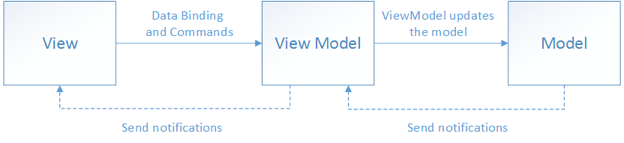
\includegraphics[width=0.8\linewidth]{figures/13_mvvm.png}
\caption{The MVVM pattern}
\label{fig:mvvm_pattern}
\end{figure}


At a high level, the view "knows about" the view model, 
and the view model "knows about" the model, but the model 
is unaware of the view model, and the view model is unaware 
of the view. Therefore, the view model isolates the view from 
the model, and allows the model to evolve independently of the view.


The separate code layers of MVVM are:
\begin{itemize}
    \item \textbf{Model}: this layer is responsible for the abstraction of the 
    data sources. Model and ViewModel work together to get and save the data.
    \item \textbf{View}: The purpose of this layer is to inform the ViewModel 
    about the user's action. This layer observes the ViewModel and does 
    not contain any kind of application logic.
    \item \textbf{ViewModel}:  It exposes those data streams which are relevant to 
    the View. Moreover, it serve as a link between the Model and the View.
\end{itemize}
\subsection{Advantages and disadvantages}
\textbf{Advantages:}
\begin{itemize}
    \item Enhance the reusability of code.
    \item All modules are independent which improves the testability of each layer.
    \item Makes project files maintainable and easy to make changes.
\end{itemize}

\textbf{Disadvantages}:
\begin{itemize}
    \item This design pattern is not ideal for small projects.
    \item If the data binding logic is too complex, the application 
    debug will be a little harder.
\end{itemize}

\subsection{Implementation and DataBinding}
There are 2 ways to implement MVVM design pattern in Android projects:
\begin{itemize}
    \item Using the \hl{DataBinding} library released by Google.
    \item Using any tool like RxJava for DataBinding. 
\end{itemize}

Google releases the Data Binding Library for Android that allows the developers 
to bind UI components in the XML layouts with the application's data repositories. 
This helps in minimizing the code of core application logic that binds with View. 
Further, Two - way Data Binding is done for binding the objects to the XML layouts 
so that object and the layout both can send data to each other. 




